\documentclass[12pt]{article}
	
	%%%%%%%%%%%%%%%%%%%%%%%%%%%%%%%%%%%%%%%%%%%%%%%%%%%%%%%%%%%%%%%%%%%%%%
	%\pdfminorversion=4
	% NOTE: To produce blinded version, replace "0" with "1" below.
	\newcommand{\blind}{0}
	
	%%%%%%% IISE Transactions margin specifications %%%%%%%%%%%%%%%%%%%
	% DON'T change margins - should be 1 inch all around.
	\addtolength{\oddsidemargin}{-.5in}%
	\addtolength{\evensidemargin}{-.5in}%
	\addtolength{\textwidth}{1in}%
	\addtolength{\textheight}{1.3in}%
	\addtolength{\topmargin}{-.8in}%
    \makeatletter
    \renewcommand\section{\@startsection {section}{1}{\z@}%
                                       {-3.5ex \@plus -1ex \@minus -.2ex}%
                                       {2.3ex \@plus.2ex}%
                                       {\normalfont\fontfamily{phv}\fontsize{16}{19}\bfseries}}
    \renewcommand\subsection{\@startsection{subsection}{2}{\z@}%
                                         {-3.25ex\@plus -1ex \@minus -.2ex}%
                                         {1.5ex \@plus .2ex}%
                                         {\normalfont\fontfamily{phv}\fontsize{14}{17}\bfseries}}
    \renewcommand\subsubsection{\@startsection{subsubsection}{3}{\z@}%
                                        {-3.25ex\@plus -1ex \@minus -.2ex}%
                                         {1.5ex \@plus .2ex}%
                                         {\normalfont\normalsize\fontfamily{phv}\fontsize{14}{17}\selectfont}}
    \makeatother
    %%%%%%%%%%%%%%%%%%%%%%%%%%%%%%%%%%%%%%%%%%%%%%%%%%%%%%%%%%%%%%%%%%%%%%%%%
	
	%%%%% IISE Transactions package list %%%%%%%%%%%%%%%%%%%%%%%%%%%%%%%%%%%%%%
	\usepackage{amsmath}
	\usepackage{graphicx}
	\usepackage{enumerate}
	\usepackage{natbib} %comment out if you do not have the package
	\usepackage{url} % not crucial - just used below for the URL
	\usepackage{hyperref}
	\documentclass{article}
    \usepackage{graphicx}
    \graphicspath{ {./images/} }

	%%%%%%%%%%%%%%%%%%%%%%%%%%%%%%%%%%%%%%%%%%%%%%%%%%%%%%%%%%%%%%%%%%%%%%%
	
	%%%%% Author package list and commands %%%%%%%%%%%%%%%%%%%%%%%%%%%%%%%%%%%%%%%%%%%%%
	%%%%% Here are some examples %%%%%%%%%%%%%%
	%	\usepackage{amsfonts, amsthm, latexsym, amssymb}
	%	\usepackage{lineno}
	%	\newcommand{\mb}{\mathbf}
	%%%%%%%%%%%%%%%%%%%%%%%%%%%%%%%%%%%%%%%%%%%%%%%%%%%%%%%%%%%%%%%%%%%%%%%%%%%%%%
	
	
	\begin{document}
		
			%%%%%%%%%%%%%%%%%%%%%%%%%%%%%%%%%%%%%%%%%%%%%%%%%%%%%%%%%%%%%%%%%%%%%%%%%%%%%%
		\def\spacingset#1{\renewcommand{\baselinestretch}%
			{#1}\small\normalsize} \spacingset{1}
		%%%%%%%%%%%%%%%%%%%%%%%%%%%%%%%%%%%%%%%%%%%%%%%%%%%%%%%%%%%%%%%%%%%%%%%%%%%%%%
		
		\if0\blind
		{
			\title{\bf PS6 Data Science}
			
			\author{ William Townsend  \\
			Department of Economics, The University of Oklahoma, Norman\\
             }
			\date{\today}
			\maketitle
		} \fi
		
		\if1\blind
		{

            \title{\bf \emph{} \LaTeX \ Template}
			\author{Author information is purposely removed for double-blind review}
			
\bigskip
			\bigskip
			\bigskip
			\begin{center}
				{\LARGE\bf \emph{IISE Transactions} \LaTeX \ Template}
			\end{center}
			\medskip
		} \fi
		\bigskip
		
%		
%	\begin{abstract}
%This document provides a \LaTeX \ template for \emph{IISE Transactions}. Your paper should be compiled in the following order: title; abstract; keywords; main text, including an introduction and a conclusion or summary; acknowledgments; declaration of interest statement; references; appendices (as appropriate). Figures and tables should be inserted into the text as close to first mention as possible (NOT appended to the end of the manuscript). In-text citations and the reference list must follow \emph{IISE Transactions} guidelines. Use 11 point font, 1 inch margins, and double-spacing for the manuscript. A typical paper for this journal should be no more than 30 pages in manuscript format, counting from the title page to references. Appendices should be included as supplemental online materials. Do not use footnotes. \emph{IISE Transactions} uses a double-blind review process. Please make sure that you submit the \textbf{blind version} of your manuscript, which does not contain any information identifying the authors.  This includes removing the authors information on the title page as well as the information that may be identifying in the Acknowledgment section. We thank you for your attention to these details.
%	\end{abstract}
%			
%	\noindent%
%	{\it Keywords:} \emph{IISE Transactions}; \LaTeX; Manuscript format; Taylor \& Francis.
%
%	%\newpage
%	\spacingset{1.5} % DON'T change the spacing!

\section{PS6a} 

\begin{document}
As a whole for this assignment, I collected homicide rate data in Mexico at the state level. I scraped the data from wikipedia and the specific site is in my R script. The data assesses homicide rates at each individual state level on an annual basis from 2006 to 2020.
The image below (PS6a) shows a linear upward trend of homicides in Mexico at the state level. Each dot is an observation representing the homicide rate per 100,000 residents in each state. The vertical axis represents homicide rates per 100,000 residents while the horizontal axis represents the years 2006 to 2020. The blue line indicates that there has been a gradual increase in homicide rates in Mexico from 2006 to 2020. In conclusion, this image shows us that Mexico is facing an overall increase in homicide rates

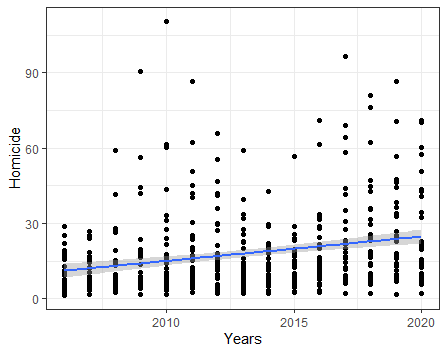
\includegraphics{PS6a_Townsend.png}

\section{PS6b}
Image PS6b (below) shows the distribution of the homicide rates per 100,000 residents over the year 2006 to 2020 at the state level. As we should expect, more areas have lower crime than vice versa. We see a right tail distribution, which shows that there is a smaller portion of Mexico that is facing comparatively more severe high homicide rates. 

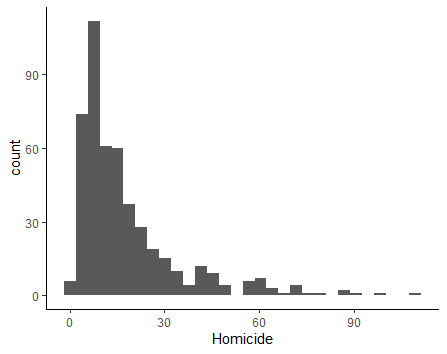
\includegraphics[]{PS6b_Townsend.png}

\section{PS6c}

The image in this section represents the distribution of homicide rates once I treat homicides as a log function. Thus, this image includes the same data as PS6b. The only difference is I logged homicides and added a value of 1 to insure my log function had no errors. In this image, we now see an image displaying something more similar to a normal distribution. Both PS6b and PS6c allow us to see what type of distribution our data displays. Such information allows us to begin assessing the data with concepts and theories that relate to normal distribution.

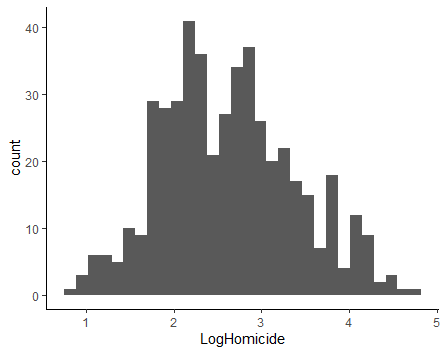
\includegraphics[]{PS6c_Townsend.png}

\end{document}





\end{document}




 
 
 





